\newpage
\section{Something Doesn't Add Up\dots}\label{A:doesntAddUp}

\fixnote{Move these to problems.}

\begin{prob}\label{P:sdau2}
Sum all the counting numbers starting with $551$ and ending at
$5051$. Use the rows of numbers below to help you.
\[
\begin{array}{c@{ + }c@{ + }c@{ + }c@{ + }c@{ + }c@{ + }c@{ + }c@{ + }c@{ + }c@{ + }c@{ + }c@{ + }c}
551 & 552 & 553 & 554 & 555 & 556 & \cdots & 5046 & 5047 & 5048 & 5049 & 5050 & 5051 \\
5051 & 5050 & 5049 & 5048 & 5047 & 5046 & \cdots & 556 & 555 & 554 & 553 & 552 & 551 
\end{array}
\]
Explain your reasoning---be sure to clearly explain what happens in
the ``dots.''  
\end{prob}


\begin{prob}\label{P:sdau1}
How many unshaded circles are in the diagram below? 
\[
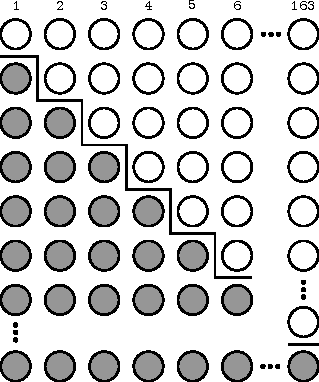
\includegraphics{../graphics/sum1.pdf}
\]
Explain your reasoning---be sure to clearly explain what happens in
the ``dots.'' Compare this with question \ref{P:sdau2}.
\end{prob}



\begin{prob}
Sum the numbers:  
\[
106 + 112 + 118 + \dots + 514
\]
Compare this with questions \ref{P:sdau1} and \ref{P:sdau2} above.
\end{prob}

\begin{prob}
Sum the numbers:
\[
2.2 + 2.9 + 3.6 + 4.3 + \dots + 81.3
\]
\end{prob}


